\documentclass{standalone}
\usepackage{ tikz }
\usepackage{ xparse }
\usepackage{../../../macros}

\begin{document}
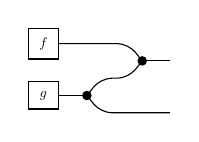
\begin{tikzpicture}[yscale=-1,x=1em,y=1.25em]
    
    \node [draw, anchor=east, minimum width=1.1em, fill=white] at (0,0) {\scalebox{0.5}{$f$}};
    \node [draw, anchor=east, minimum width=1.1em, fill=white] at (0,1.5) {\scalebox{0.5}{$g$}};

    \draw [rounded corners] (0,0) -- (2.5,0) -- (3,0.5);
    \draw [rounded corners] (0,1.5) -- (1,1.5);
    \filldraw (1,1.5) circle (1.5pt);
    \draw [rounded corners] (1,1.5) -- (1.5,1) -- (2.5,1) -- (3,0.5);
    \filldraw (3,0.5) circle (1.5pt);
    \draw (3,0.5) -- (4,0.5);
    \draw [rounded corners] (1,1.5) -- (1.5,2) -- (4,2);

\end{tikzpicture}
\end{document}